\documentclass[12pt,a4paper]{article}
\usepackage{geometry}
\geometry{left=2.5cm,right=2.5cm,top=2.0cm,bottom=2.5cm}
\usepackage[english]{babel}
\usepackage{amsmath,amsthm}
\usepackage{amsfonts}
\usepackage[longend,ruled,linesnumbered]{algorithm2e}
\usepackage{fancyhdr}
\usepackage{ctex}
\usepackage{array}
\usepackage{listings}
\usepackage{color}
\usepackage{graphicx}

\begin{document}


\title{
《优化理论与算法》第 2 次作业
}

\date{}

\author{
姓名：\underline{焦传斌}~~~~~~
学号：\underline{2024111223}~~~~~~}

\maketitle
\maketitle
	\begin{itemize}
\item 作业截止于{\bf 周五（3/20/2026）}，在Canvas系统中提交PDF或照片文件
\item 作业题目的tex文件可以在Canvas中下载
\item 鼓励相互讨论，但不要抄袭.
\end{itemize}
	%%%%%%%%%%%%%%%%%%%%%%%%%%%%%%%%%%%%%%%%%%%%%%%%%%%%%%%%%%%%%%%%%
	%%%%%%%%%%%%%%%%%%%%%%%%%%%%%%%%%%%%%%%%%%%%%%%%%%%%%%%%%%%%%%%%%
	


\section{复习与积累}
\paragraph{1.1}
\begin{itemize}
\item 阅读Bertsimas and Tsitsikils，也就是Introduction to Linear Optimization教材，第一章相关内容。
\item  收看同名超星线上慕课，课程章节4.2内容，快速预习单纯形法相关内容。
\end{itemize}

\section{习题}


\paragraph{2.1}
设矩阵 $ A $ 为：
\[
A = \begin{bmatrix} 
3 & 2  \\
2 & 4 
\end{bmatrix}
\]

\begin{enumerate}
    \item $A$矩阵的特征值是什么？
    \item 如何将$A$矩阵对角化？($A=U\Lambda U^T$，其中$U$为正交矩阵)
    \item $A$是否为正定矩阵？
\end{enumerate}

\textbf{解：}
\begin{enumerate}

\item 求解特征方程：
\[
\det\begin{pmatrix} 3-\lambda & 2 \\ 2 & 4-\lambda \end{pmatrix} = 0
\]
化简得：
\[
\lambda^2 - 7\lambda + 8 = 0
\]
解得特征值：
\[
\lambda_1 = \frac{7+\sqrt{17}}{2}, \qquad \lambda_2 = \frac{7-\sqrt{17}}{2}
\]

\item 矩阵 $A$ 的对角化形式为 $A = U\Lambda U^T$，其中 $\Lambda$ 是包含特征值的对角矩阵，$U$ 是包含特征向量的矩阵。

对于 $\lambda_1 = \dfrac{7+\sqrt{17}}{2}$，解方程 $(A-\lambda_1 I)\mathbf{x}=\mathbf{0}$ 得特征向量：
\[
\mathbf{x}_1 = \begin{bmatrix} 1 \\[4pt] \dfrac{-1-\sqrt{17}}{4} \end{bmatrix}
\]

对于 $\lambda_2 = \dfrac{7-\sqrt{17}}{2}$，解方程 $(A-\lambda_2 I)\mathbf{x}=\mathbf{0}$ 得特征向量：
\[
\mathbf{x}_2 = \begin{bmatrix} 1 \\[4pt] \dfrac{-1+\sqrt{17}}{4} \end{bmatrix}
\]

特征向量矩阵 $U$：
\[
U = \begin{bmatrix}
1 & 1 \\[6pt]
\dfrac{-1-\sqrt{17}}{4} & \dfrac{-1+\sqrt{17}}{4}
\end{bmatrix}
\]

对角矩阵 $\Lambda$：
\[
\Lambda = \begin{bmatrix}
\dfrac{7+\sqrt{17}}{2} & 0 \\[6pt]
0 & \dfrac{7-\sqrt{17}}{2}
\end{bmatrix}
\]

对角化结果：
\[
A = U\Lambda U^T
\]

\item 判断矩阵是否正定的方法是看其所有特征值是否均大于零。

由第\,1\,题，矩阵 $A$ 的特征值为：
\[
\lambda_1 = \frac{7+\sqrt{17}}{2} > 0, \qquad \lambda_2 = \frac{7-\sqrt{17}}{2} > 0
\]
由于两个特征值均大于零，因此矩阵 $A$ \textbf{是正定矩阵}。

\end{enumerate}

	%%%%%%%%%%%%%%%%%%%%%%%%%%%%%%%%%%%%%%%%%%%%%%%%%%%%%%%%%%%%%%%%%
	%%%%%%%%%%%%%%%%%%%%%%%%%%%%%%%%%%%%%%%%%%%%%%%%%%%%%%%%%%%%%%%%%
	


\paragraph{2.2}

下列约束是否是线性约束？如果不是线性约束，能否将其等价转换成线性约束？如果能转化，请展示；如果不能，说明原因。
\begin{enumerate}
	
	\item $ -3x_1-5x_2+22 \geq 18$
	
	\item $2x_1^2 -8 \leq 0$
	
	\item $x_1x_2-3x_1-x_2+3=0$
	
	\item $\frac{3x_1-2x_2}{2x_1+1} = 4$
	
	\item $e^{3x_1+5x_2} \geq 12$
	
	\item $|x| \leq 3$
	
	\item $\max\{x_1, -x_1+7x_2, x_2^3\} \leq 8$
	
	\item $\min\{2x_1,3x_2\} \geq \max\{10-x_1,6-x_2\}$
	
	
\end{enumerate}

\textbf{解：}
\begin{enumerate}

\item $-3x_1-5x_2+22\ge 18$ 是线性约束。化简得
\[
3x_1+5x_2\le 4
\]

\item $2x_1^2-8\le 0$ 不是线性约束，因为含有二次项 $x_1^2$。但可等价转化为
\[
x_1^2\le 4 \quad\Longleftrightarrow\quad -2\le x_1\le 2 \quad\Longleftrightarrow\quad x_1\ge 
-2,\quad x_1\le 2
\]

\item $x_1x_2-3x_1-x_2+3=0$ 不是线性约束，因为含有乘积项 $x_1x_2$。原式等价于
\[
(x_1-1)(x_2-3)=0 \quad\Longleftrightarrow\quad x_1=1 \quad\text{或}\quad x_2=3
\]
这表示两条直线的并集，不能等价转化为线性约束。

\item $\dfrac{3x_1-2x_2}{2x_1+1}=4$ 不是线性约束，因为变量出现在分母中。移项得
\[
3x_1-2x_2=4(2x_1+1) \quad\Longrightarrow\quad 5x_1+2x_2=-4
\]
但还必须满足 $2x_1+1\ne 0$。其中 $5x_1+2x_2=-4$ 是线性的，但条件 $2x_1+1\ne 0$ 不是线性约束，因此不能等价转化为线性约束。

\item $e^{3x_1+5x_2}\ge 12$ 不是线性约束，因为含有指数函数。由于指数函数单调递增，可等价转化为
\[
3x_1+5x_2\ge \ln 12
\]
可等价转化为线性约束。

\item $|x|\le 3$ 不是线性约束，因为含有绝对值。但可等价转化为
\[
-3\le x\le 3 \quad\Longleftrightarrow\quad x\ge -3,\quad x\le 3
\]

\item $\max\{x_1,\,-x_1+7x_2,\,x_2^3\}\le 8$ 不是线性约束，因为含有 $\max$ 和三次项 $x_2^3$。由
\[
\max\{a,b,c\}\le 8 \iff a\le 8,\; b\le 8,\; c\le 8
\]
原约束等价于 $x_1\le 8$，$-x_1+7x_2\le 8$，$x_2^3\le 8$。又因为立方函数单调递增，$x_2^3\le 8\iff x_2\le 2$，故原约束等价于
\[
x_1\le 8,\qquad -x_1+7x_2\le 8,\qquad x_2\le 2
\]
可等价转化为线性约束。

\item $\min\{2x_1,3x_2\}\ge\max\{10-x_1,6-x_2\}$ 不是线性约束，因为含有 $\min$ 和 $\max$。
由 $\min\{a,b\}\ge\max\{c,d\}$ 等价于 $a\ge c,\;a\ge d,\;b\ge c,\;b\ge d$，得
\begin{align*}
2x_1 &\ge 10-x_1 \implies x_1\ge\dfrac{10}{3}\\
2x_1 &\ge 6-x_2  \implies 2x_1+x_2\ge 6\\
3x_2 &\ge 10-x_1 \implies x_1+3x_2\ge 10\\
3x_2 &\ge 6-x_2  \implies x_2\ge\dfrac{3}{2}
\end{align*}
故可等价转化为线性约束。

\end{enumerate}

\paragraph{2.3}
将下列线性规划转换成标准型
\begin{equation*}
	\begin{aligned}
	\text{minimize}  & -x_1&+7x_2 &+3x_3 &\\
	\text{subject to}& x_1 &+3x_2  &-2x_3    &\leq 0 \\
	&x_1 &+4x_2  &-2x_3  &\geq 0  \\
	&-x_1 &+2x_2  &+3x_3    &=  5  \\
	&x_1 \leq 0, &x_2 \geq 0, &x_3  \text{无约束}&  
	\end{aligned}
\end{equation*}

\textbf{解：}

设 $x_1=-x_4$，$x_3=x_5-x_6$，$x_4,x_5,x_6\ge 0$，再引入松弛变量 $x_7\ge0$ 和剩余变量 $x_8\ge0$，则原问题化为标准型：
\begin{equation*}
\begin{aligned}
\text{minimize}   \quad & x_4+7x_2+3x_5-3x_6 \\
\text{subject to} \quad
& -x_4+3x_2-2x_5+2x_6+x_7 = 0 \\
& -x_4+4x_2-2x_5+2x_6-x_8 = 0 \\
&  x_4+2x_2+3x_5-3x_6       = 5 \\
& x_2,x_4,x_5,x_6,x_7,x_8\ge 0
\end{aligned}
\end{equation*}


\paragraph{2.4}
课件"lp2工业生产案例"的P29中总结了允许延迟交付的模型。此模型没有考虑物料清单树的影响，也就是生产量$x_{ij}$只消耗产能，相互之间不作为生产的物料消耗。

请问在考虑物料清单树的情况下，如何修改此模型的一般形式？（注：可以假设已知参数$u_{i'i}$表述生产1单位物料$i'$消耗物料$i$的数量。）

\textbf{解：}

\textbf{集合定义：}
\begin{itemize}
    \item $I$：物料集合
    \item $F \subseteq I$：有外部需求的成品集合
    \item $J = \{1, 2, \dots, T\}$：计划期集合
\end{itemize}

\textbf{参数：}
\begin{itemize}
    \item $p_i$：生产 1 单位物料 $i$ 所需产能
    \item $P_j$：第 $j$ 期可用产能
    \item $d_{ij}$：第 $j$ 期物料 $i$ 的外部需求
    \item $r_{ij}$：第 $j$ 期物料 $i$ 的单位延期交付成本
    \item $s_i$：物料 $i$ 的初始库存
    \item $u_{i'i}$：生产 1 单位物料 $i'$ 消耗物料 $i$ 的数量
\end{itemize}

\textbf{决策变量：}
\begin{itemize}
    \item $x_{ij} \ge 0$：第 $j$ 期生产的物料 $i$ 数量
    \item $y_{ij} \ge 0$：第 $j$ 期期末物料 $i$ 的库存量
    \item $z_{ij} \ge 0$：第 $j$ 期物料 $i$ 的交付量
    \item $\delta_{ij} \ge 0$：第 $j$ 期期末物料 $i$ 的延期交付量
\end{itemize}

\textbf{模型：}

目标函数（最小化延期交付成本）：
\[
\min \sum_{i \in F} \sum_{j \in J} r_{ij} \delta_{ij}
\]

约束条件：

(1) 产能约束：
\[
\sum_{i \in I} p_i x_{ij} \le P_j, \qquad \forall j \in J
\]

(2) 库存平衡约束（考虑物料清单树）：
\[
y_{ij} = y_{i,j-1} + x_{ij} - z_{ij} - \sum_{i' \in I} u_{i'i} x_{i'j}, \qquad \forall i \in I,\ j \in J
\]

(3) 延期交付递推：
\[
\delta_{ij} = \delta_{i,j-1} + d_{ij} - z_{ij}, \qquad \forall i \in F,\ j \in J
\]

(4) 初始条件：
\[
y_{i0} = s_i, \qquad \forall i \in I
\]
\[
\delta_{i0} = 0, \qquad \forall i \in F
\]

(5) 非负约束：
\[
x_{ij},\ y_{ij},\ z_{ij},\ \delta_{ij} \ge 0
\]

\textbf{进一步考虑生产提前期：}

若物料 $i$ 的提前期为 $t_i$，则第 $j$ 期真正完工入库的数量不是 $x_{ij}$，而是之前某一期投产的数量。记第 $j$ 期物料 $i$ 的完工入库量为：
\[
q_{ij} = x_{i,j-t_i+1}
\]
当 $j - t_i + 1 \le 0$ 时，约定 $q_{ij} = 0$。

此时库存平衡约束修改为：
\[
y_{ij} = y_{i,j-1} + x_{i,j-t_i+1} - z_{ij} - \sum_{i' \in I} u_{i'i} x_{i'j}, \qquad \forall i \in I,\ j \in J
\]

其余约束保持不变。

\paragraph{2.5}
Bertsimas and Tsitsikils 书中第一章课后题 1.15
(hint: (b) if one or both elements are not easy to incorporate into the linear programming formulation, you might consider integer decision variables or nonlinear constraints.)

\textbf{解：}

\textbf{(a) 线性规划模型}

设 $x_1$ 为每天生产的第一种产品数量，$x_2$ 为每天生产的第二种产品数量。第一种产品每件利润为 $9-1.2=7.8$，第二种产品每件利润为 $8-0.9=7.1$。

目标函数（最大化每日利润）及约束条件为：
\[
\begin{aligned}
\max\quad & 7.8x_1+7.1x_2\\
\text{s.t.}\quad
& \frac{1}{4}x_1+\frac{1}{3}x_2\le 90,\\
& \frac{1}{8}x_1+\frac{1}{3}x_2\le 80,\\
& x_1,x_2\ge 0.
\end{aligned}
\]

\textbf{(b) 两种修改的讨论}

\textbf{(i) 最多可安排 50 小时组装加班，成本为每小时 7 美元}

此要素\textbf{可以很容易纳入线性规划模型}。设 $y$ 表示每天使用的加班组装工时，则 $0\le y\le 50$，组装工时约束改为 $\dfrac{1}{4}x_1+\dfrac{1}{3}x_2\le 90+y$，目标函数改为
\[
\max\ z=7.8x_1+7.1x_2-7y
\]
该修改仍然是线性规划。

\textbf{(ii) 若每日原材料账单超过 300 美元，则原材料享受 10\% 折扣}

原材料账单为 $m=1.2x_1+0.9x_2$，若超过 300 美元则成本变为 $0.9m$。此要素\textbf{不容易直接纳入普通线性规划}，因为存在阈值触发的分段成本，下面给出两种处理方法。

\textbf{方法一：分两种情况分别求解}

\textit{情况 1：不享受折扣}（$1.2x_1+0.9x_2\le 300$）
\[
\begin{aligned}
\max\quad & 7.8x_1+7.1x_2\\
\text{s.t.}\quad
& \frac{1}{4}x_1+\frac{1}{3}x_2\le 90,\\
& \frac{1}{8}x_1+\frac{1}{3}x_2\le 80,\\
& 1.2x_1+0.9x_2\le 300,\\
& x_1,x_2\ge 0.
\end{aligned}
\]

\textit{情况 2：享受折扣}（$1.2x_1+0.9x_2> 300$），折扣后利润系数为 $9-0.9\times1.2=7.92$，$8-0.9\times0.9=7.19$（其中 $\varepsilon>0$ 为极小正数）：
\[
\begin{aligned}
\max\quad & 7.92x_1+7.19x_2\\
\text{s.t.}\quad
& \frac{1}{4}x_1+\frac{1}{3}x_2\le 90,\\
& \frac{1}{8}x_1+\frac{1}{3}x_2\le 80,\\
& 1.2x_1+0.9x_2\ge 300+\varepsilon,\\
& x_1,x_2\ge 0.
\end{aligned}
\]
分别求出两个线性规划的最优值，取较优者即可。

\textbf{方法二：建立混合整数线性规划}

引入 0-1 变量 $b\in\{0,1\}$（$b=0$ 不打折，$b=1$ 打折），辅助变量 $w$（打折时的原材料账单），以及足够大的常数 $M$，则模型为：
\[
\max\ 9x_1+8x_2-m+0.1w
\]
\[
\begin{aligned}
\text{s.t.}\quad
& \frac{1}{4}x_1+\frac{1}{3}x_2\le 90,\\
& \frac{1}{8}x_1+\frac{1}{3}x_2\le 80,\\
& m=1.2x_1+0.9x_2,\\
& m\le 300+Mb,\\
& m\ge (300+\varepsilon)b,\\
& 0\le w\le Mb,\\
& w\le m,\\
& w\ge m-M(1-b),\\
& x_1,x_2\ge 0,\\
& b\in\{0,1\}.
\end{aligned}
\]
当 $b=0$ 时 $w=0$（不打折）；当 $b=1$ 时 $w=m$（节省 $0.1m$）。

\textbf{结论：}加班组装工时可以很容易纳入线性规划模型；原材料折扣不容易直接纳入普通线性规划，可通过分情况求解或改用混合整数线性规划处理。

\paragraph{2.6}
课件"运筹学简介"的P20中介绍了不能完全可分情况下的支持向量机的建模方法。请随机生成10个2维点作为A集合，再随机生成10个2维点作为B集合。建立课件所示线性规划模型，利用COPT求解此问题最优解。提交资料：

\begin{itemize}
	\item 绘制图像：画出A、B集合中的所有点和优化求解所得分隔线（如课件图所示），
	
	\item 代码打印附在作业后面
\end{itemize}


（注：在随机生成的2维点$(x_1,x_2)$过程中，可以自己定义A集合和B集合点的区间，点在区间内可以是均匀分布。只要生成结果是课件中不可分情况就可以）

\textbf{解：}

\textbf{1. 线性规划模型}

根据题目要求，建立如下线性规划模型：

设 $A$ 集合点为 $x_i$（$i=1,2,\ldots,10$），$B$ 集合点为 $y_j$（$j=1,2,\ldots,10$），分隔线为 $a^Tz+b=0$。

引入松弛变量 $\delta_i=(1-a^Tx_i-b)^+$ 和 $\sigma_j=(a^Ty_j+b+1)^+$，则问题转化为：

\[
\begin{aligned}
\min \quad & \sum_{i=1}^{10}\delta_i+\sum_{j=1}^{10}\sigma_j\\
\text{s.t.} \quad
& a^Tx_i+b+\delta_i\ge 1, \quad \forall i=1,\ldots,10,\\
& a^Ty_j+b-\sigma_j\le -1, \quad \forall j=1,\ldots,10,\\
& \delta_i,\sigma_j\ge 0.
\end{aligned}
\]

\textbf{2. 数据生成}

采用随机均匀分布生成数据点：
\begin{itemize}
\item 在区域 $[0, 3.5]\times[0, 3.5]$ 中随机生成 A 集合的 10 个点
\item 在区域 $[2, 5.5]\times[2, 5.5]$ 中随机生成 B 集合的 10 个点
\end{itemize}


\textbf{3. 求解结果}

使用 COPT 求解器求解上述线性规划问题，得到最优解：

\[
\begin{aligned}
a_1 &= -1.98\\
a_2 &= -0.35\\
b &= 6.33
\end{aligned}
\]

分隔线方程为：
\[
-1.98x_1 - 0.35x_2 + 6.33 = 0
\]

目标函数值（总分类错误）为 $6.71$。

\textbf{4. 可视化结果}

图像如下所示，其中蓝色圆圈表示 A 集合的点，红色叉号表示 B 集合的点，绿色实线为求解得到的分隔线，绿色虚线为支持向量边界线。
\begin{figure}[h]
\centering
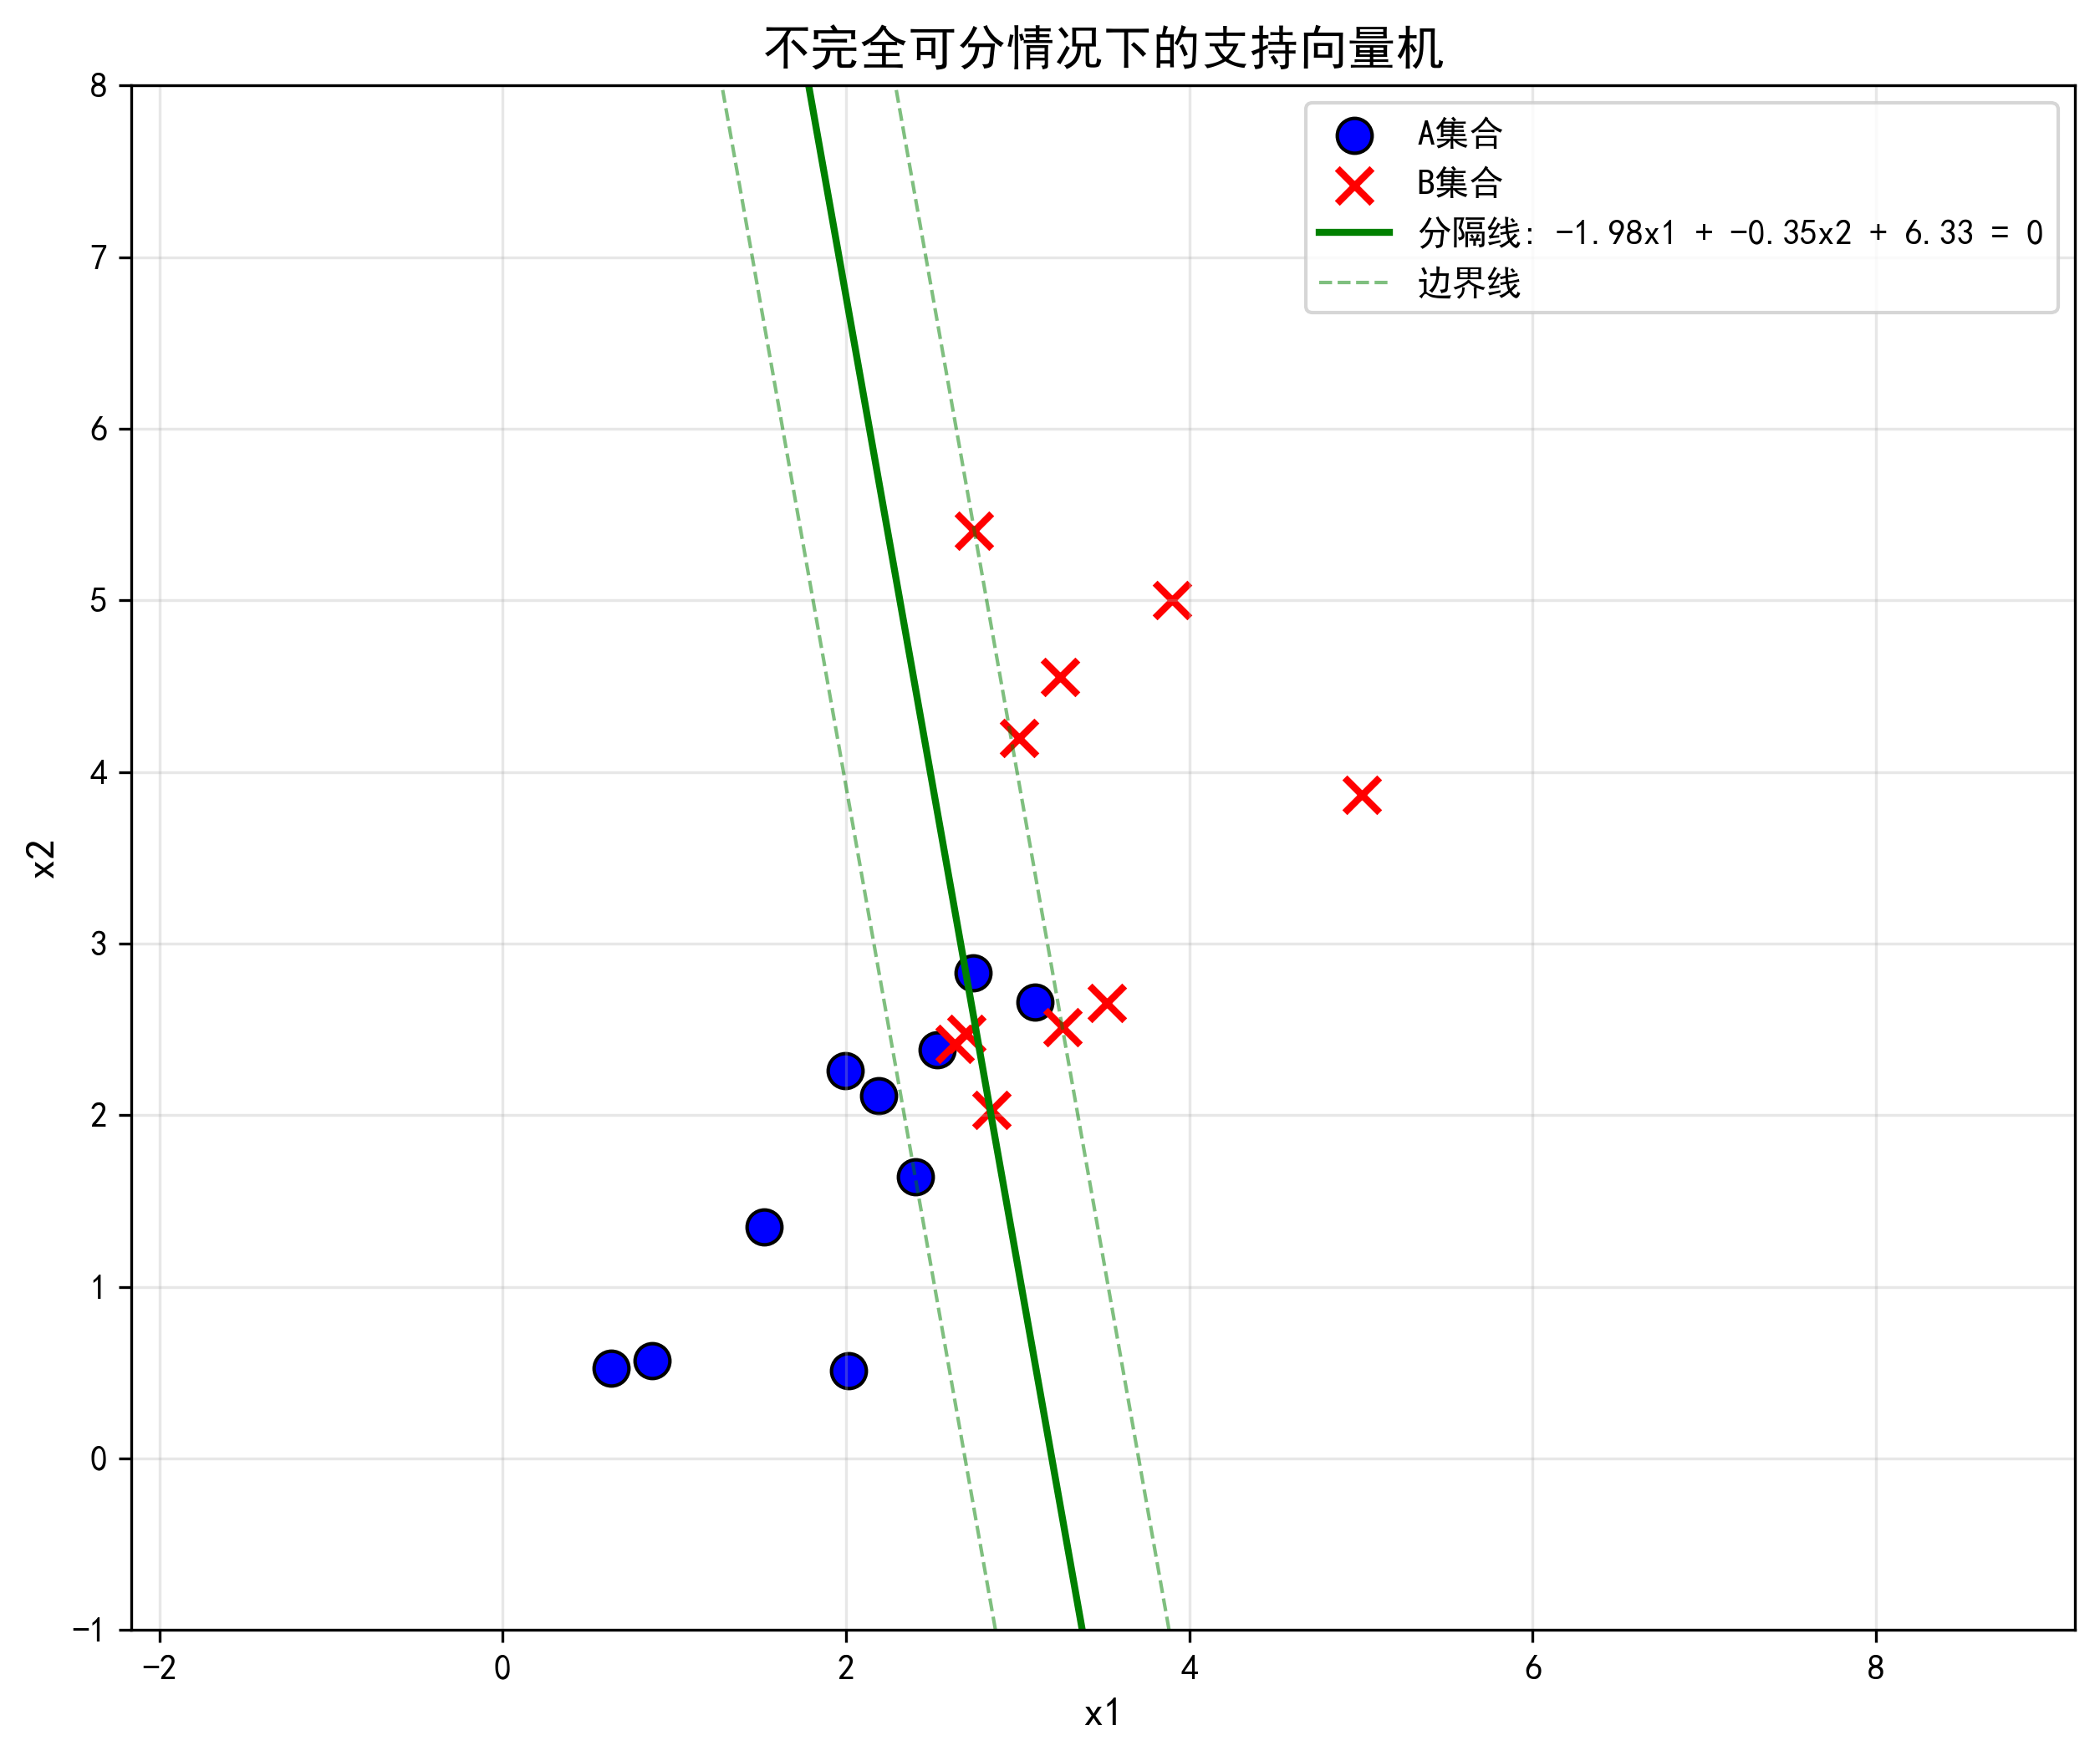
\includegraphics[width=0.8\textwidth]{svm_result.png}
\caption{不完全可分情况下的支持向量机求解结果}
\end{figure}

\newpage

\textbf{5. Python 代码}

\begin{lstlisting}[language=Python, basicstyle=\small\ttfamily, breaklines=true, frame=single]
import numpy as np
import matplotlib.pyplot as plt
from coptpy import COPT, Envr

plt.rcParams['font.sans-serif'] = ['SimHei', 'Microsoft YaHei', 'SimSun']
plt.rcParams['axes.unicode_minus'] = False

np.random.seed(456)

A = np.random.uniform(0, 3.5, (10, 2))
B = np.random.uniform(2, 5.5, (10, 2))

print("A集合的点：")
print(A)
print("\nB集合的点：")
print(B)

# 创建COPT环境和模型
env = Envr()
model = env.createModel("SVM")

# 决策变量
a1 = model.addVar(lb=-COPT.INFINITY, ub=COPT.INFINITY, name="a1")
a2 = model.addVar(lb=-COPT.INFINITY, ub=COPT.INFINITY, name="a2")
b = model.addVar(lb=-COPT.INFINITY, ub=COPT.INFINITY, name="b")

# 松弛变量
delta = []
for i in range(len(A)):
    delta.append(model.addVar(lb=0, name=f"delta_{i}"))

sigma = []
for j in range(len(B)):
    sigma.append(model.addVar(lb=0, name=f"sigma_{j}"))

# 目标函数
model.setObjective(sum(delta) + sum(sigma), COPT.MINIMIZE)

# 约束条件
for i in range(len(A)):
    model.addConstr(a1 * A[i][0] + a2 * A[i][1] + b + delta[i] >= 1,
                    name=f"A_constraint_{i}")

for j in range(len(B)):
    model.addConstr(a1 * B[j][0] + a2 * B[j][1] + b - sigma[j] <= -1,
                    name=f"B_constraint_{j}")

model.solve()

if model.status == COPT.OPTIMAL:
    a1_opt = a1.x
    a2_opt = a2.x
    b_opt = b.x
    
    print(f"\n最优解：")
    print(f"a1 = {a1_opt:.4f}")
    print(f"a2 = {a2_opt:.4f}")
    print(f"b = {b_opt:.4f}")
    print(f"目标函数值（总分类错误）= {model.objval:.4f}")
    
    print(f"\n分隔线方程：{a1_opt:.4f} * x1 + {a2_opt:.4f} * x2 + {b_opt:.4f} = 0")
    
    # 绘制图像
    plt.figure(figsize=(10, 8))
    
    # 绘制A集合的点（蓝色圆圈）
    plt.scatter(A[:, 0], A[:, 1], c='blue', marker='o', s=100,
                label='A集合', edgecolors='black')
    
    # 绘制B集合的点（红色叉号）
    plt.scatter(B[:, 0], B[:, 1], c='red', marker='x', s=100,
                label='B集合', linewidths=2)
    
    # 绘制分隔线 a1*x1 + a2*x2 + b = 0
    x1_range = np.linspace(-1, 8, 100)
    if abs(a2_opt) > 1e-6:
        x2_line = -(a1_opt * x1_range + b_opt) / a2_opt
        plt.plot(x1_range, x2_line, 'g-', linewidth=2,
                label=f'分隔线: {a1_opt:.2f}x1 + {a2_opt:.2f}x2 + {b_opt:.2f} = 0')
        
        # 绘制支持向量边界
        x2_upper = -(a1_opt * x1_range + b_opt - 1) / a2_opt
        x2_lower = -(a1_opt * x1_range + b_opt + 1) / a2_opt
        plt.plot(x1_range, x2_upper, 'g--', linewidth=1, alpha=0.5,
                label='边界线')
        plt.plot(x1_range, x2_lower, 'g--', linewidth=1, alpha=0.5)
    
    plt.xlabel('x1', fontsize=12)
    plt.ylabel('x2', fontsize=12)
    plt.title('不完全可分情况下的支持向量机', fontsize=14, fontweight='bold')
    plt.legend(fontsize=10)
    plt.grid(True, alpha=0.3)
    plt.axis('equal')
    plt.xlim(-1, 8)
    plt.ylim(-1, 8)
    
    plt.savefig('svm_result.png', dpi=300, bbox_inches='tight')
    print("\n图像已保存为 svm_result.png")
    
    plt.show()
else:
    print(f"求解失败，状态码：{model.status}")
\end{lstlisting}

\end{document}